\documentclass{article}
\usepackage[utf8]{inputenc}
\usepackage{minted}
\usepackage{hyperref}
\usepackage{amsmath,amssymb}
\usepackage{graphicx}


\title{\begin{center}CSE 5370: Bioinformatics Homework-1\end{center}}
\author{Divya Boggavarapu}
\date{September 2022}

\begin{document}

\maketitle

\subsection*{Collaboration Statement}
I have collaborated with Vijitha Kotapati(1001860730) and Tulasi Sridevi Navuluru(1002010740) to do the programming questions in 1.2, 1.3 and 1.4  by understanding the Fisher's exact test and Bonferroni Correction concepts.

\section{Genome Wide Association Studies (GWAS)}

You are working as a population geneticist for the government of a large country
trying to understand associations between a complex genetic trait (phenotype)
and genetic variants in a sequencing study conducted on hundreds of volunteer
participants.
  In this study, there are 50 patients in the case cohort and 100 people in the
control cohort. For these participants, 1000 particular SNPs (snp 1, snp 2, ...,
snp 1000) are measured and reported (in a real-world study, number of SNPs
tested can be several million). These SNPs are either C-alleles or T-alleles. You
are required to conclude whether there is significant evidence whether any of
the C-allele SNPs contribute to a person’s risk of developing the complex trait
(Note: this question may be challenging to complete prior to the walk through
lecture).


\subsection{Generating Your Own Unique Data}
We are provided with a python script named datasetGenerator.py. This program will take in our UTA student ID as an argument and generates a unique artificial dataset of the mentioned study. To run the code, simply run:
\begin{itemize}
             \gg { \textbf{\textit{python3 datasetGenerator.py --ID 1002086719}}}
\\
\end{itemize}

Running the program will create a file named 1002086719.csv in the same directory this program is located in. This data set has 1000 rows rep- resenting each SNP and 5 columns representing the name of the SNP, number of C-alleles in the case cohort, number of T-alleles in the case cohort, number of C-alleles in the control cohort, and number of T-alleles in the control cohort.
 





\subsection{Fisher’s Exact Test}
In this scenario, you can represent the data as contingency tables and the effect
sizes as odds ratios (please refer to the walk through lecture and slides). For
each SNP, if there is significant evidence that the odds ratio for allele C is higher
than 1, you can conclude that allele C is among the causes of the complex genetic trait.
The Fisher’s exact test is a statistical test performed on the contingency
tables and tests whether the odds ratio of the underlying populations are close to
1 or not. Using the scipy’s fisher exact function, find the p-value associated
with each SNP for your data set. Assuming an effective p-value of 5 \times {10^{-8}}$, which SNPs can be considered statistically significant regarding the complex genetic trait? Based on the documentation of fisher exact function, you need to explain what the null hypothesis of this test is and what it means. Also you need to choose to explain how you choose the alternative argument in
this function. You have to provide a file named results.csv containing the
p-values for each SNP in the first column and the SNPs that are significant in
the second column. You should also report the number of significant SNPs in
your written answer.
            \begin{itemize}
    \item The SNPs with odds ratio for allele C that is higher than 1 is considered to be statistically significant regarding the complex genetic trait.

    \begin{itemize}
    \item Explain what the null hypothesis of this test is and what it means. \end{itemize}
    \begin{itemize}
        \item \textbf{Null Hypothesis} $H_{0}$ = \textbf{Allele C is among the causes of the complex genetic
trait.}
        
        \item \textbf{Alternate Hypothesis} $H_{1}$ = \textbf{Allele C is not the cause of the complex genetic
trait.}  
The Null Hypothesis H0 adopted for this test means that if allele C causes complex genetic trait when the odds ratio for allele C is higher than 1.\end{itemize}  
\item  I have chosen less in the alternative argument in fisher exact function. I have chosen my Alternative hypothesis $H_{1}$ as allele c is not the cause of the complex genetic trait which makes odd ratio to be less than 1. We use less as the argument in fisher's exact when the odds ratio of the underlying population is less than one. Hence I have used less as the alternative argument.
\item The total number of significant SNPs is \textbf{166}}
   
\end{itemize}


\subsection {Corrected P-Values}
{Assuming each association between a SNP and the phenotype is an independent hypothesis, and we want our effective p-value to be 5 × 10−8
          What is our Bonferroni-corrected p-value? How many SNPs are significant 		            under the corrected p-value? }
           
         
\begin{itemize}
        \item \textbf{\textbf{}\textbf{}The Bonferroni-corrected p-value is $\frac{\alpha}{n} = \frac{5\times10^-8}{1000} = 5 \times {10^{-11}}$}\item \textbf{The total number of corrected P values are  119}}
\\  
\\
\subsection{Manhattan Plots}
\begin{itemize}
    \textbf{Generate a psuedo Manhattan plot of the −log10 (p − values) with the original and corrected p-value threshold illustrated. Include a paragraph describing what the Manhattan plot shows.}\\   
  
   \\
    \\

\begin{document}
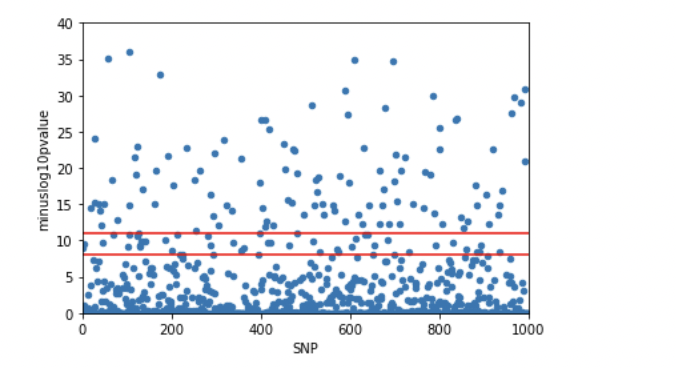
\includegraphics[BioHomeWork1]{Matplotlib}

\\
\item  \item The X axis in the plot represents SNPs and Y axis represents the associated p values as −log10 (p). The blue dots in the plot represents the scattered p values for respective SNPs. The plots between lines represents the threshold.
\end{itemize}
% referred https://www.overleaf.com/learn/latex for the latex concepts and referred https://www.python-graph-gallery.com/manhattan-plot-with-matplotlib for manhatten plot.



\section{Difficulty Adjustment}
Your answers to this section will be used to adjust the difficulty of future assignments in the class. 
\begin{itemize}
    \item  How long did this assignment take you to complete?
    \begin{itemize}
        \item \textbf{I completed my assignment in 14 hours.}
    \end{itemize}
    \item  If the assignment took you longer than the 10 hours, which parts were overly difficult?
    \begin{itemize}
        \item \textbf{The Documentation, understanding the question and designing took around 5 hrs . Its challenging yet very interesting to work on this assignment}
    \end{itemize}
\end{itemize}

\end{document}
\end{document}